% questions.tex —— 2015 年·全国Ⅱ卷·理科 · 题目内容片段（无答案）
% 由 tools/generate_projects.py 依来源总账自 2015/2015_数学真题_全国2理_试题.md 生成，勿手改（改源 MD 后重跑）


\begin{gktip}
按固定来源照录。题图为TikZ源图描绘，布局坐标与未标数据不作精确数值；原卷未印满分、时长或小题分值，不补写。
\end{gktip}

\gkpart{一、选择题}

\begin{question}
\gkti{1}已知集合 $A=\{-2,-1,0,1,2\}$，$B=\{x\mid (x-1)(x+2)<0\}$，则 $A\cap B$ 等于（　）

(A) $\{-1,0\}$　(B) $\{0,1\}$　(C) $\{-1,0,1\}$　(D) $\{0,1,2\}$

\end{question}
\begin{question}
\gkti{2}若 $a$ 为实数，且 $(2+ai)(a-2i)=-4i$，则 $a=$（　）

(A) $-1$　(B) $0$　(C) $1$　(D) $2$

\Needspace{0.4\textheight}
\end{question}
\begin{question}
\gkti{3}根据下面给出的 2004 年至 2013 年我国二氧化硫年排放量（单位：万吨）柱形图，以下结论中不正确的是（　）
\nopagebreak[4]
\begin{center}% Source p.1 (965). Heights below are visual layout only, not measured emissions.
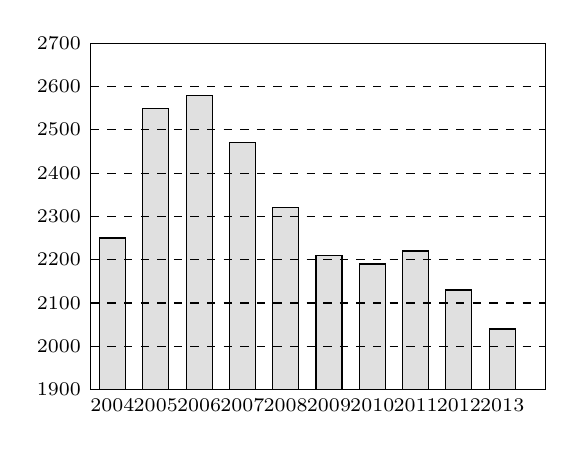
\begin{tikzpicture}[x=.55cm,y=.55cm,font=\scriptsize,line width=.4pt]
  \foreach \i/\h in {0/3.5,1/6.5,2/6.8,3/5.7,4/4.2,5/3.1,6/2.9,7/3.2,8/2.3,9/1.4}
    \draw[fill=black!12] (\i+.2,0) rectangle (\i+.8,\h);
  \foreach \j in {1,...,7} \draw[dashed] (0,\j)--(10.5,\j);
  \draw (0,0) rectangle (10.5,8);
  \foreach \j in {0,...,8} {
    \pgfmathtruncatemacro{\lab}{1900+100*\j}
    \node[left] at (0,\j) {\lab};
  }
  \foreach \i in {0,...,9} {
    \pgfmathtruncatemacro{\lab}{2004+\i}
    \node[below] at (\i+.5,0) {\lab};
  }
\end{tikzpicture}
\end{center}
\nopagebreak[4]
(A) 逐年比较，2008 年减少二氧化硫排放量的效果最显著  
(B) 2007 年我国治理二氧化硫排放显现成效  
(C) 2006 年以来我国二氧化硫年排放量呈减少趋势  
(D) 2006 年以来我国二氧化硫年排放量与年份正相关

\end{question}
\begin{question}
\gkti{4}已知等比数列 $\{a_n\}$ 满足 $a_1=3$，$a_1+a_3+a_5=21$，则 $a_3+a_5+a_7=$（　）

(A) $21$　(B) $42$　(C) $63$　(D) $84$

\end{question}
\begin{question}
\gkti{5}设函数
$\displaystyle f(x)=\begin{cases}1+\log_2(2-x),&x<1,\\2^{x-1},&x\geqslant1,\end{cases}$
则 $f(-2)+f(\log_2 12)=$（　）

(A) $3$　(B) $6$　(C) $9$　(D) $12$

\Needspace{0.4\textheight}
\end{question}
\begin{question}
\gkti{6}一个正方体被一个平面截去一部分后，剩余部分的三视图如图，则截去部分体积与剩余部分体积的比值为（　）
\nopagebreak[4]
\begin{center}% Source p.1 (965): no view titles or extra dimensions.
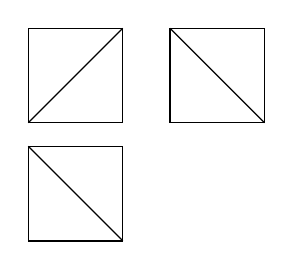
\begin{tikzpicture}[line width=.45pt]
  \draw (0,1.5) rectangle (1.2,2.7);
  \draw (0,1.5)--(1.2,2.7);
  \draw (1.8,1.5) rectangle (3,2.7);
  \draw (1.8,2.7)--(3,1.5);
  \draw (0,0) rectangle (1.2,1.2);
  \draw (0,1.2)--(1.2,0);
\end{tikzpicture}
\end{center}
\nopagebreak[4]
(A) $\dfrac18$　(B) $\dfrac17$　(C) $\dfrac16$　(D) $\dfrac15$

\end{question}
\begin{question}
\gkti{7}过三点 $A(1,3)$，$B(4,2)$，$C(1,-7)$ 的圆交 $y$ 轴于 $M,N$ 两点，则 $|MN|=$（　）

(A) $2\sqrt6$　(B) $8$　(C) $4\sqrt6$　(D) $10$

\Needspace{0.4\textheight}
\end{question}
\begin{question}
\gkti{8}下边程序框图的算法思路源于我国古代数学名著《九章算术》中的“更相减损术”。执行该程序框图，若输入的 $a,b$ 分别为 $14,18$，则输出的 $a=$（　）
\nopagebreak[4]
\begin{center}% Source p.1 (965). Paths are drawn explicitly; no extra TikZ libraries required.
\begin{tikzpicture}[x=1cm,y=1cm,font=\small,line width=.45pt,>=stealth]
  \draw[rounded corners=3pt] (-.4,0) rectangle (.4,.48);
  \node at (0,.24) {开始};
  \draw[->] (0,0)--(0,-.4);
  \draw (-.7,-.4)--(.85,-.4)--(.7,-.9)--(-.85,-.9)--cycle;
  \node at (0,-.65) {输入 $a,b$};
  \draw[->] (0,-.9)--(0,-1.35);
  \draw (0,-1.35)--(1.1,-1.6)--(0,-1.85)--(-1.1,-1.6)--cycle;
  \node at (0,-1.6) {$a\ne b$};
  \draw[->] (-1.1,-1.6)--(-1.6,-1.6)--(-1.6,-2.2);
  \node[above] at (-1.12,-1.6) {是};
  \draw[->] (1.1,-1.6)--(1.6,-1.6)--(1.6,-2.2);
  \node[above] at (1.12,-1.6) {否};
  \draw (-1.6,-2.2)--(-.6,-2.45)--(-1.6,-2.7)--(-2.6,-2.45)--cycle;
  \node at (-1.6,-2.45) {$a>b$};
  \draw[->] (-2.6,-2.45)--(-3,-2.45)--(-3,-2.95);
  \node[above] at (-2.65,-2.45) {是};
  \draw[->] (-.6,-2.45)--(-.2,-2.45)--(-.2,-2.95);
  \node[above] at (-.55,-2.45) {否};
  \draw (-3.7,-2.95) rectangle (-2.3,-3.4);
  \node at (-3,-3.175) {$a=a-b$};
  \draw (-.9,-2.95) rectangle (.5,-3.4);
  \node at (-.2,-3.175) {$b=b-a$};
  \draw (-3,-3.4)--(-3,-3.65)--(-.2,-3.65)--(-.2,-3.4);
  \draw[->] (-1.6,-3.65)--(-1.6,-3.9)--(-4.05,-3.9)--(-4.05,-1.12)--(0,-1.12);
  \draw (.98,-2.2)--(2.34,-2.2)--(2.18,-2.7)--(.82,-2.7)--cycle;
  \node at (1.58,-2.45) {输出 $a$};
  \draw[->] (1.58,-2.7)--(1.58,-3.15);
  \draw[rounded corners=3pt] (1.18,-3.15) rectangle (1.98,-3.63);
  \node at (1.58,-3.39) {结束};
\end{tikzpicture}
\end{center}
\nopagebreak[4]
(A) $0$　(B) $2$　(C) $4$　(D) $14$

\end{question}
\begin{question}
\gkti{9}已知 $A,B$ 是球 $O$ 的球面上两点，$\angle AOB=90^\circ$，$C$ 为该球面上的动点，若三棱锥 $O-ABC$ 体积的最大值为 $36$，则球 $O$ 的表面积为（　）

(A) $36\pi$　(B) $64\pi$　(C) $144\pi$　(D) $256\pi$

\Needspace{0.4\textheight}
\end{question}
\begin{question}
\gkti{10}如图，长方形 $ABCD$ 的边 $AB=2$，$BC=1$，$O$ 是 $AB$ 的中点，点 $P$ 沿着边 $BC,CD$ 与 $DA$ 运动，记 $\angle BOP=x$。将动点 $P$ 到 $A,B$ 两点距离之和表示为 $x$ 的函数 $f(x)$，则 $y=f(x)$ 的图象大致为（　）
\nopagebreak[4]
\begin{center}% Source p.1 (965). P is a schematic position on DC.
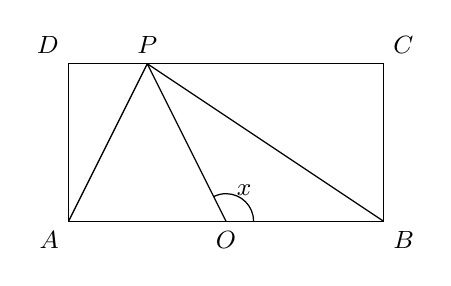
\begin{tikzpicture}[line width=.45pt,font=\small]
  \coordinate (A) at (0,0); \coordinate (B) at (4,0);
  \coordinate (C) at (4,2); \coordinate (D) at (0,2);
  \coordinate (O) at (2,0); \coordinate (P) at (1,2);
  \draw (A)--(B)--(C)--(D)--cycle;
  \draw (A)--(P)--(B) (P)--(O);
  \draw (2.35,0) arc[start angle=0,end angle=116.565,radius=.35];
  \node at (2.23,.39) {$x$};
  \node[below left] at (A) {$A$}; \node[below right] at (B) {$B$};
  \node[above right] at (C) {$C$}; \node[above left] at (D) {$D$};
  \node[below] at (O) {$O$}; \node[above] at (P) {$P$};
\end{tikzpicture}
\end{center}
\nopagebreak[4]
\nopagebreak[4]
\begin{center}% Source p.1 (965). Qualitative option; all unlabelled ordinates are layout only.
\begin{tikzpicture}[x=1cm,y=1cm,font=\small,line width=.45pt,>=stealth]
  \draw[->] (0,0)--(3.3,0) node[right] {$x$};
  \draw[->] (0,0)--(0,3.2) node[above left] {$y$};
  \node[below left] at (0,0) {$O$};
  \node[left] at (0,1.55) {$2$};
  \foreach \u/\lab in {.65/{\frac{\pi}{4}},1.3/{\frac{\pi}{2}},1.95/{\frac{3\pi}{4}},2.6/{\pi}} {
    \draw (\u,0)--(\u,.06);
    \node[below] at (\u,0) {$\lab$};
  }
  \draw (0,1.55)--(.65,2.5)--(1.3,2.18)--(1.95,2.5)--(2.6,1.55);
  \node[anchor=north east] at (-.12,-.38) {(A)};
\end{tikzpicture}
\end{center}
\nopagebreak[4]
\nopagebreak[4]
\begin{center}% Source p.1 (965). Qualitative option; all unlabelled ordinates are layout only.
\begin{tikzpicture}[x=1cm,y=1cm,font=\small,line width=.45pt,>=stealth]
  \draw[->] (0,0)--(3.3,0) node[right] {$x$};
  \draw[->] (0,0)--(0,3.2) node[above left] {$y$};
  \node[below left] at (0,0) {$O$};
  \node[left] at (0,1.55) {$2$};
  \foreach \u/\lab in {.65/{\frac{\pi}{4}},1.3/{\frac{\pi}{2}},1.95/{\frac{3\pi}{4}},2.6/{\pi}} {
    \draw (\u,0)--(\u,.06);
    \node[below] at (\u,0) {$\lab$};
  }
  \draw (0,1.55) .. controls (.30,1.58) and (.48,2.1) .. (.65,2.5)
    .. controls (1.0,2.1) and (1.6,2.1) .. (1.95,2.5)
    .. controls (2.13,1.95) and (2.32,1.58) .. (2.6,1.55);
  \node[anchor=north east] at (-.12,-.38) {(B)};
\end{tikzpicture}
\end{center}
\nopagebreak[4]
\nopagebreak[4]
\begin{center}% Source p.1 (965). Qualitative option; all unlabelled ordinates are layout only.
\begin{tikzpicture}[x=1cm,y=1cm,font=\small,line width=.45pt,>=stealth]
  \draw[->] (0,0)--(3.3,0) node[right] {$x$};
  \draw[->] (0,0)--(0,3.2) node[above left] {$y$};
  \node[below left] at (0,0) {$O$};
  \node[left] at (0,1.55) {$2$};
  \foreach \u/\lab in {.65/{\frac{\pi}{4}},1.3/{\frac{\pi}{2}},1.95/{\frac{3\pi}{4}},2.6/{\pi}} {
    \draw (\u,0)--(\u,.06);
    \node[below] at (\u,0) {$\lab$};
  }
  \draw (0,1.55)--(1.3,2.22)--(2.6,1.55);
  \node[anchor=north east] at (-.12,-.38) {(C)};
\end{tikzpicture}
\end{center}
\nopagebreak[4]
\nopagebreak[4]
\begin{center}% Source p.1 (965). Qualitative option; all unlabelled ordinates are layout only.
\begin{tikzpicture}[x=1cm,y=1cm,font=\small,line width=.45pt,>=stealth]
  \draw[->] (0,0)--(3.3,0) node[right] {$x$};
  \draw[->] (0,0)--(0,3.2) node[above left] {$y$};
  \node[below left] at (0,0) {$O$};
  \node[left] at (0,1.55) {$2$};
  \foreach \u/\lab in {.65/{\frac{\pi}{4}},1.3/{\frac{\pi}{2}},1.95/{\frac{3\pi}{4}},2.6/{\pi}} {
    \draw (\u,0)--(\u,.06);
    \node[below] at (\u,0) {$\lab$};
  }
  \draw (0,1.55) .. controls (0,3.15) and (2.6,3.15) .. (2.6,1.55);
  \node[anchor=north east] at (-.12,-.38) {(D)};
\end{tikzpicture}
\end{center}
\nopagebreak[4]
\end{question}
\begin{question}
\gkti{11}已知 $A,B$ 为双曲线 $E$ 的左、右顶点，点 $M$ 在 $E$ 上，$\triangle ABM$ 为等腰三角形，且顶角为 $120^\circ$，则 $E$ 的离心率为（　）

(A) $\sqrt5$　(B) $2$　(C) $\sqrt3$　(D) $\sqrt2$

\end{question}
\begin{question}
\gkti{12}设函数 $f'(x)$ 是奇函数 $f(x)$（$x\in\mathbb R$）的导函数，$f(-1)=0$，当 $x>0$ 时，$xf'(x)-f(x)<0$，则使得 $f(x)>0$ 成立的 $x$ 的取值范围是（　）

(A) $(-\infty,-1)\cup(0,1)$　(B) $(-1,0)\cup(1,+\infty)$  
(C) $(-\infty,-1)\cup(-1,0)$　(D) $(0,1)\cup(1,+\infty)$

\end{question}
\gkpart{二、填空题}

\begin{question}
\gkti{13}设向量 $\boldsymbol a,\boldsymbol b$ 不平行，向量 $\lambda\boldsymbol a+\boldsymbol b$ 与 $\boldsymbol a+2\boldsymbol b$ 平行，则实数 $\lambda=$\gkblank{}。

\end{question}
\begin{question}
\gkti{14}若 $x,y$ 满足约束条件 $\begin{cases}x-y+1\geqslant0,\\x-2y\leqslant0,\\x+2y-2\leqslant0,\end{cases}$ 则 $z=x+y$ 的最大值为\gkblank{}。

\end{question}
\begin{question}
\gkti{15}$(a+x)(1+x)^4$ 的展开式中 $x$ 的奇数次幂项的系数之和为 $32$，则 $a=$\gkblank{}。

\end{question}
\begin{question}
\gkti{16}设 $S_n$ 是数列 $\{a_n\}$ 的前 $n$ 项和，且 $a_1=-1$，$a_{n+1}=S_nS_{n+1}$，则 $S_n=$\gkblank{}。

\end{question}
\gkpart{三、解答题}

\begin{question}
\gkti{17}在 $\triangle ABC$ 中，$D$ 是 $BC$ 上的点，$AD$ 平分 $\angle BAC$，$\triangle ABD$ 面积是 $\triangle ADC$ 面积的 $2$ 倍。

(1) 求 $\dfrac{\sin B}{\sin C}$；  
(2) 若 $AD=1$，$DC=\dfrac{\sqrt2}{2}$，求 $BD$ 和 $AC$ 的长。

\Needspace{0.4\textheight}
\end{question}
\begin{question}
\gkti{18}某公司为了解用户对其产品的满意度，从 $A,B$ 两地区分别随机调查了 $20$ 个用户，得到用户对产品的满意度评分如下：

```text
A 地区：62  73  81  92  95  85  74  64  53  76
        78  86  95  66  97  78  88  82  76  89
B 地区：73  83  62  51  91  46  53  73  64  82
        93  48  65  81  74  56  54  76  65  79
```

(1) 根据两组数据完成两地区用户满意度评分的茎叶图，并通过茎叶图比较两地区用户满意度评分的平均值及分散程度（不要求计算出具体值，给出结论即可）；
\nopagebreak[4]
\begin{center}% Source p.1 (965). Printed blank template: do not insert leaves.
\begin{tikzpicture}[font=\small,line width=.45pt]
  \draw (-4,0)--(4,0);
  \draw (-.25,.48)--(-.25,-2.9);
  \draw (.25,.48)--(.25,-2.9);
  \node[above] at (-2.1,0) {$A$ 地区};
  \node[above] at (2.1,0) {$B$ 地区};
  \foreach \stem/\y in {4/-.25,5/-.75,6/-1.25,7/-1.75,8/-2.25,9/-2.75}
    \node at (0,\y) {\stem};
\end{tikzpicture}
\end{center}
\nopagebreak[4]
(2) 根据用户满意度评分，将用户的满意度从低到高分为三个等级：

\begin{center}
\begin{tabular}{llll}
\toprule
满意度评分 & 低于 $70$ 分 & $70$ 分到 $89$ 分 & 不低于 $90$ 分 \\
\midrule
满意度等级 & 不满意 & 满意 & 非常满意 \\
\bottomrule
\end{tabular}
\end{center}

记事件 $C$：“$A$ 地区用户的满意度等级高于 $B$ 地区用户的满意度等级”。假设两地区用户的评价结果相互独立。根据所给数据，以事件发生的频率作为相应事件发生的概率，求 $C$ 的概率。

\Needspace{0.4\textheight}
\end{question}
\begin{question}
\gkti{19}如图，长方体 $ABCD-A_1B_1C_1D_1$ 中，$AB=16$，$BC=10$，$AA_1=8$，点 $E,F$ 分别在 $A_1B_1,D_1C_1$ 上，$A_1E=D_1F=4$。过点 $E,F$ 的平面 $\alpha$ 与此长方体的面相交，交线围成一个正方形。

(1) 在图中画出这个正方形（不必说明画法和理由）；  
(2) 求直线 $AF$ 与平面 $\alpha$ 所成角的正弦值。
\nopagebreak[4]
\begin{center}% Source p.2 (966). AF is already dashed in source; requested square is absent.
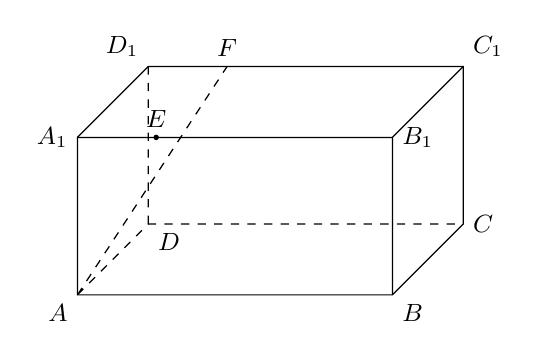
\begin{tikzpicture}[line width=.45pt,font=\small]
  \coordinate (A) at (0,0); \coordinate (B) at (4,0);
  \coordinate (C) at (4.9,.9); \coordinate (D) at (.9,.9);
  \coordinate (A1) at (0,2); \coordinate (B1) at (4,2);
  \coordinate (C1) at (4.9,2.9); \coordinate (D1) at (.9,2.9);
  \coordinate (E) at (1,2); \coordinate (F) at (1.9,2.9);
  \draw (A)--(B)--(C)--(C1)--(D1)--(A1)--cycle;
  \draw (A1)--(B1)--(C1) (B)--(B1);
  \draw[dashed] (A)--(D)--(C) (D)--(D1) (A)--(F);
  \fill (E) circle (1pt);
  \node[below left] at (A) {$A$}; \node[below right] at (B) {$B$};
  \node[right] at (C) {$C$}; \node[below right] at (D) {$D$};
  \node[left] at (A1) {$A_1$}; \node[right] at (B1) {$B_1$};
  \node[above right] at (C1) {$C_1$}; \node[above left] at (D1) {$D_1$};
  \node[above] at (E) {$E$}; \node[above] at (F) {$F$};
\end{tikzpicture}
\end{center}
\nopagebreak[4]
\end{question}
\begin{question}
\gkti{20}已知椭圆 $C:9x^2+y^2=m^2$（$m>0$），直线 $l$ 不过原点 $O$ 且不平行于坐标轴，$l$ 与 $C$ 有两个交点 $A,B$，线段 $AB$ 的中点为 $M$。

(1) 证明：直线 $OM$ 的斜率与 $l$ 的斜率的乘积为定值；  
(2) 若 $l$ 过点 $\left(\dfrac m3,m\right)$，延长线段 $OM$ 与 $C$ 交于点 $P$，四边形 $OAPB$ 能否为平行四边形？若能，求此时 $l$ 的斜率；若不能，说明理由。

\end{question}
\begin{question}
\gkti{21}设函数 $f(x)=e^{mx}+x^2-mx$。

(1) 证明：$f(x)$ 在 $(-\infty,0)$ 单调递减，在 $(0,+\infty)$ 单调递增；  
(2) 若对于任意 $x_1,x_2\in[-1,1]$，都有 $|f(x_1)-f(x_2)|\leqslant e-1$，求 $m$ 的取值范围。

\Needspace{0.4\textheight}
\end{question}
\begin{question}
\gkti{22}如图，$O$ 为等腰三角形 $ABC$ 内一点，$\odot O$ 与 $\triangle ABC$ 的底边 $BC$ 交于 $M,N$ 两点，与底边上的高 $AD$ 交于点 $G$，且与 $AB,AC$ 分别相切于 $E,F$ 两点。

(1) 证明：$EF\parallel BC$；  
(2) 若 $AG$ 等于 $\odot O$ 的半径，且 $AE=MN=2\sqrt3$，求四边形 $EBCF$ 的面积。
\nopagebreak[4]
\begin{center}% Source p.2 (966). Tangency is preserved by a layout construction, not solution data.
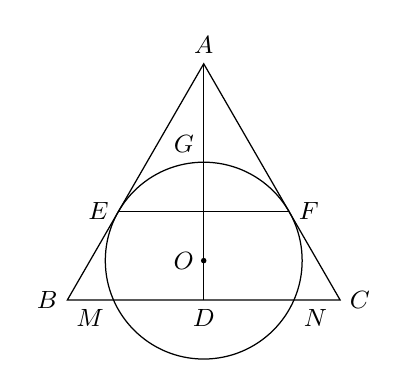
\begin{tikzpicture}[line width=.45pt,font=\small]
  \coordinate (A) at (0,3); \coordinate (B) at (-1.732,0);
  \coordinate (C) at (1.732,0); \coordinate (D) at (0,0);
  \coordinate (O) at (0,.5); \coordinate (G) at (0,1.75);
  \coordinate (E) at (-1.0825,1.125); \coordinate (F) at (1.0825,1.125);
  \coordinate (M) at (-1.1456,0); \coordinate (N) at (1.1456,0);
  \draw (A)--(B)--(C)--cycle;
  \draw (A)--(D) (E)--(F);
  \draw (O) circle (1.25);
  \fill (O) circle (1pt);
  \node[above] at (A) {$A$}; \node[left] at (B) {$B$};
  \node[right] at (C) {$C$}; \node[below] at (D) {$D$};
  \node[left] at (O) {$O$}; \node[above left] at (G) {$G$};
  \node[left] at (E) {$E$}; \node[right] at (F) {$F$};
  \node[below left] at (M) {$M$}; \node[below right] at (N) {$N$};
\end{tikzpicture}
\end{center}
\nopagebreak[4]
\end{question}
\begin{question}
\gkti{23}在直角坐标系 $xOy$ 中，曲线 $C_1:\begin{cases}x=t\cos\alpha,\\y=t\sin\alpha,\end{cases}$（$t$ 为参数，$t\ne0$），其中 $0\leqslant\alpha<\pi$。在以 $O$ 为极点，$x$ 轴正半轴为极轴的极坐标系中，曲线 $C_2:\rho=2\sin\theta$，$C_3:\rho=2\sqrt3\cos\theta$。

(1) 求 $C_2$ 与 $C_3$ 交点的直角坐标；  
(2) 若 $C_1$ 与 $C_2$ 相交于点 $A$，$C_1$ 与 $C_3$ 相交于点 $B$，求 $|AB|$ 的最大值。

\end{question}
\begin{question}
\gkti{24}已知 $a,b,c,d$ 均为正数，且 $a+b=c+d$，证明：

(1) 若 $ab>cd$，则 $\sqrt a+\sqrt b>\sqrt c+\sqrt d$；  
(2) $\sqrt a+\sqrt b>\sqrt c+\sqrt d$ 是 $|a-b|<|c-d|$ 的充要条件。

\end{question}